 \documentclass[9pt, twocolumn,twoside]{gsajnl}
% how i want it for inport into word: \documentclass[9pt, onecolumn,twoside]{gsajnl}
% how i want it for pdf: \documentclass[9pt,twocolumn,twoside,lineno]{gsajnl}
% Use the documentclass option 'lineno' to view line numbers

\usepackage{epstopdf}
\usepackage{wrapfig}
\usepackage[T1]{fontenc}
\usepackage[latin1]{inputenc}
\articletype{inv}
\runningtitle{Soy scientific manuscript} % For use in the footer
\runningauthor{Connelly \textit{et al.}}

\title{Soybeans for the Future: Population Genetic Analysis Of A Historical Swedish Soybean Population For Future Germpasm Utalisation}


%Swedish Soybean Genetic Diversity: Influence of Breeding Practices and Identification of Selection Signatures

%Genetic Diversity in a Swedish Soybean Population: Signatures of Selection and Implications for Future Soybean Breeding in Northern Environments

% Swedish Soybean Genetic Diversity: Influence of Breeding Practices and Identification of Selection Signatures

%Soybean Genetic Variation in Swedish population: A Study of Breeding Influence and Selection Signatures

%Swedish Soybean Genetic Diversity: Influence of Breeding Practices and Identification of Selection Signatures

%Genetic Diversity in the Swedish Soybean Population: Impacts of the Breeding Program, Selection Signatures, and Implications for Future Germplasm Utilization

%Population Genetic Insights into the Swedish Soybean Population: Impact of Breeding Strategies and Selection Signatures


\author[1,$\ast$]{Josephine Estelle Ananda Connelly}
\author[2,$\dagger$]{Guillaume Paul Ramstein}
\author[3,$\dagger$]{Wolf L Eiserhardt}
\author[4,$\dagger$]{Torben Asp}


\affil[1,2,4]{Centre for Quantitative Genetics and Genomics, Faculty of Technical Sciences, Aarhus University (DK).}
\affil[1,3]{Department of Biology, Faculty of Natural Sciences, Aarhus University, (DK).}
\affil[3]{Royal Botanic Gardens, Kew, (UK).}

\affil[$\dagger$]{These authors share senior authorship}
\correspondingauthoraffiliation[$\ast$]{Corresponding author: AU, josephineconnelly@qgg.au.dk.}

\begin{abstract}
Soybean (Glycine max L. Merrill) is the world's leading oilseed crop used as a  primary source of vegetable oil for human consumption and protein meal for animal feed. 
A breeding program of the 1940s-1970s resulted in 160 accessions later donated to the seed bank of the Nordic Genetic Resource Center (NordGen). Climate change and plant protein independence have driven the idea of trying to repeat the effort of plant genetic enhancement for soybean cultivation in northwest Europe. Uncovering the population genetics of this as yet unutilised germplasm can give a head start to these future soybean breeding efforts. The Swedish soybeans are revealed as a population that has undergone bottlenecks, resulting in reduced effective population size (Ne), elevated levels of genetic drift, decreased nucleotide diversity, and increased linkage, all attributed to the selective breeding efforts or the selection of the genetic progenitors.  

The Core collection (CCA) was created by \cite{haupt20}  as a collection identified from the USDA germplasm for central European soybean breeding. Comparison of the CCA to the Swedish breeding program accessions (SBPA) has been used throughout the paper to put the SBPA into the perspective of germplasm likely to be utilised in these future soybean breeding efforts. The SBPA has half the nucleotide diversity of the CCA. Fst analysis for population subdivision reveals a population difference of 0.22 calculated for a weighted Fst estimate.
 
genomic regions of selection differentiation were detected between the CCA and the SBPA by using snp specific genomewide pairwise Fst and to uncover 

The reduced level of genetic variation in elite breeding populations means that in the case of soybean, there is a need to increase germplasm utilization for abiotic adaptation to the colder conditions of Northern Europe. This research means to examine the genetic structure and diversity within a population of soybeans originating from a breeding program during the 1940s to 1970s in Sweden (SBPA). We aim to gain insights into the pressures that have shaped the genetic makeup of these soybean accessions. So that this resource of untold potential can be fully utilized.  

   

\end{abstract}

\keywords{Soybean; Glycine max; Population Genetics; Diversity; Fst; Linkage Disequalibrium; Selection Signatures; Plant Breeding}

\dates{\rec{29 09, 2023} \acc{29 09, 2023}}

\begin{document}

\maketitle
\thispagestyle{firststyle}
\vspace{-13pt}

\section{Introduction}

This is a link to part A where there is the extensive introduction/litterature review:
https://www.overleaf.com/2689273778mwyzpfmjvbmf

ps abrtract is in the preamble...

Soybean is Glycine max, this and that and important.

Several severe genetic bottlenecks occurred in soybean during domestication and the continuous breeding efforts. Compared to the wild species, the genetic diversity was halved, resulting in a loss of 81\% of rare alleles (Hyten et al., 2006). Additionally, two major bottlenecks occurred during the development of North American modern cultivars, where only a few landraces were used and as a result of intensive soybean breeding over the past 75 years. Elite cultivars have emerged, but they are derived from only about 19 landraces. Consequently, the North American breeding pools now retain only 72\% of genome diversity and have lost 79\% of rare alleles found in diverse landraces \cite{gizlice96}.

soybean needs to be grown in the north:

With the European Green Deal of 2019, there is an intention of harnessing the potential of EU plant protein production. This intention is motivated as a response to the needs of farmers, producers and consumers. 
The production and sourcing of plant-based proteins in the EU also carries with it a range of environmental benefits such as a decrease in imports and therefore transport pollution reduction. 

The difficulties identified by the Report: Development of plant proteins in the European Union \cite{EC18} are:

- the agronomic conditions in Europe, which are not optimal for large-scale production of plant proteins; 
- the economic profitability of these crops in Europe; 
- the competitiveness of EU protein crops compared to imported plant proteins; 
- competition over the use of arable land; 
- and a lack of research on breeding, agronomic practices and different uses. 

(Danish field trials have shown the Swedish cultivar Fiskeby V to yield only 11.2hkg/ha \cite{petersen09,petersen10}. Modern soybean breeding has led to yield increases of $229 \, \text{kg} \, ha^{-1} \, \text{yr}^{-1}$ \cite{rincker14}, advancing and adapting soybean cultivation even further. )

Expanding the production of soy to the northern climates by leveraging the advancements in soybean breeding and focusing on the genes relevant to adaptation can diversify the global supply chain, reduce dependency, and potentially alleviate the environmental pressures associated with soy production in high biodiversity, sensitive areas/ecologically vulnerable regions. With the global demand for soy and the need for sustainable agricultural practices, investing in breeding programs to develop soybean varieties suitable for northern climates can present a promising part of the solution. 

\textit{the Swedish soybeans (goals and scope)}
The Swedish breeding population SBPA consists of the soybean germplasm collection from the seed bank of the Nordic Genetic Resource Center (NordGen). One of the cultivars that resulted from this breeding program is well-known as a genetic source of 
goals
not technical

scope

\textit{In this study}

In this study, we present insights into the population genetic analysis of the soybean accessions obtained from the NorGen genebank accessions. 
There haven't been any past investigations into this germplasm resource, so therefore, the goal of this project was to better understand the value of the genebank collection so as to help precipitate the utilisation of these soybean genetic resources. to increase germplasm utilization through understanding what we have in the genebanks. We present population stratification, diversity and linkage of the population. Through population genetic analyses supported by breeders publications and historical documents, we can infer what happened and what  to this population and determine the genetic significance of the resource. 
Presented is a comprehensive population genetic analysis of the SBPA soybean population. Determining the genetic diversity and population structure of the SBPA. An assessment of how the SBPA compare to the broader genetic diversity in the species through a comparative analysis with a core collection (CCA). 
And a test of selection efficacy of the Swedish breeding program by screening biological pathways. 




\section{Materials and methods}
\label{sec:materials:methods}

\subsection{Swedish Breeding Program Collection}
155 soybean accessions were obtained from the Nordgen genebank of Swedish origin. These accessions originate from a Swedish breeding program (SBP) running from the 1840s to the 1970s, which used material consisting of a mixture of elite cultivars of the time and Japanese/Siberian landraces, breeding for the adaptation to the cool climate of northwestern Europe \cite{holmberg1973}. The Swedish breeding program (SBP) of the 1940s-1980s of Algot Holmberg and Sons from Norrkoping produced the known cultivars Fiskeby III, Fiskeby V, Träff, and Bråvalla, which are included in the NordGen gene bank accessions and in this analysis excluding Fiskeby III that was not available from the Nordgen genebank at the time.

\subsection{The Core Collection}
The Core Collection (CCA) consists of two samplings of the core collection from haupt20. A 5\% and 10\% collection with overlapping accessions in total consisting of 409 accessions after filtering. 
The Core collection accessions (CCA) used here is a subset of the large soybean germplasm collection, the  USDA genebank accessions consisting of 415 of the USDA soy germplasm accessions. This Core collection has been selected with a focus on adaptation to high-latitude cold regions using environmental data from phenotypic trials in Germany and comparing Donor opulation of Environments (DPE) in Asia and the Target Population of Environments (TPE) in Central Europe by \cite{haupt20}. From the more than 17.000 accessions, two diverse core collections of 183 and 366 accessions were created. These 514 diversity panels are used here due to that they are likely preadapted to cultivation in Central Europe while simultaneously conserving a high level of genetic diversity. 

\subsection{The Founders Collection}
The USDA Soybean Germplasm Collection maintains accessions of >17000 cultivated soybeans and is part of the U.S. National Plant Germplasm System (NPGS).  These accessions have been previously genotyped with the SoySNP50K iSelect BeadChip  \cite{song13,song15} has been used for genotyping the USDA Soybean Germplasm Collection and is available for use from SoyBase (https://soybase.org/) in the version mapped to the soybean genome assembly Glyma.Wm82.a2  \cite{schmutz10}. In the pedigree information from Nordgen SBPA, there are 10 accessions present in the USDA genebank and thus are part of the SoySNP50K genotypic data. These specific accessions were included as they are considered Founders of the SBP. 

\textit{DNA extraction and sequencing information?:}

\subsection{Genotyping and filtering of whole genome sequence SNP}
The accessions from the Nordgen genebank and the Core collection accessions were whole genome sequenced. Four of the Core collection seeds didn't germinate in time for the sequencing, resulting in accessions sequenced 574. Of the Nordgen accessions, Four were of Latvian origin and therefore excluded in further analysis. 
The reads were aligned to the Williams 82 2a reference genome \cite{schmutz10} using an adapted GATK Best Practices \cite{mckenna10}, keeping MQ30 and biallelic sites and using VCFtools v. 0.1.16 \cite{danecek11} applying a minor allele frequency (MAF) filter of 0.01 in order to remove rare variants from the data, reducing the number of SNPs markers were initially called (raw dataset) from 17,648,123 to 10,000,122. 
For a detailed account of accessions, programs and commands used see supplementary material: \nameref{sec:supplementary:material} 
A further three accessions were removed due to missing phenotype data and a single accession that had missing data > 5$\%$ using BCFtools \cite{danecek21}, resulting in 153 Swedish accessions from the NordGen genebank and 409 of the CCA accessions. Five per cent missing data at SNPs was also removed resulting in an SNP count of 8,533,444. This data set was used to compare the Allele Frequency of the two populations. For all other analyses, MAF 5\%  was removed using VCFtools (--maf 0.05) on the dataset as a whole, except for the case of LD calculation MAF5\% was removed separately for SBPA and CCA.  

\subsection{SNP intersect }
An intersection was made of the whole genome sequenced data (153 SBPA and 409 CCA) and the SoySNP50K array data of the 10 Founders.  This was done using BCFtools with the command "isec". The intersecting data was 35.486 SNPs. 

For a detailed account of programs and commands, see supplementary material, \nameref{sec:supplementary:material} (S3: Methods 1) data preparation and filtering and \nameref{sec:data:availability} for data. 

* here insert a table with information of the snps and stuff.

\subsection{Population Structure Analysis}
To infer population stratification of the Swedish accessions from the NordGen gene bank and the Core collection and of the 12 accessions assumed to be founders of the Swedish breeding program. Principal component analysis (PCA) on SNP genotype data was applied using the package SnpRelate in R (A Parallel Computing Toolset for Relatedness and Principal Component Analysis of SNP Data). The functions in SNPRelate for PCA used (snpgdsPCA) calculate the genetic covariance matrix from genotypes, computing the correlation coefficients between sample loadings and genotypes for each SNP and SNP eigenvectors were calculated. The WGS data was used for a number of the PCA, and where the possible genetic Founders to the Swedish breeding program the intersect data is used and indicated in figures; \ref{fig:pca}.

The package SNPRelate in R was used to compute an identity-by-state (IBS) matrix that calculates the proportion that two randomly selected reads that contain a certain SNP locus are the same or different between two individuals. The resulting pairwise IBS matrix was used to conduct a hierarchical cluster analysis to generate a dendrogram using the function \textit{snpgdsHCluster: Hierarchical cluster analysis In SNPRelate }in R. 

F-statistics, particularly Fst, quantifies the distribution of genetic diversity by measuring the variation in allele frequencies among different populations. 
Relatedness measures F-statistics (also known as fixation indices) for given populations were calculated using the function \textit{snpgdsFst: F-statistics (fixation indices) in SNPRelate }in R. The whole genome data was used to calculate the pairwise population differentiation measured in the populations of the Swedish accessions as a subpopulation with the Core Collection as a representation of the total population. Fst is comparing the expected heterozygosity in the subpopulation (HS) to that expected in the total population (HT) :

$F_{\text{ST}} = 1 - \left(\frac{H_{\text{S}}}{H_{\text{T}}}\right)$

\subsection{Genetic Diversity Estimates}
The idea is to look into the effects of the bottleneck caused by the SBP, the increased drift and will be detected as a reduction of Ne. Detecting a decrease in genetic diversity as a measure of allele frequency, nucleotide diversity and LD increase. Allele Frequency (AF) was calculated using Vcftools --freq and plotted in R. LD analysis was preformed in VCFtools  --maf 0.05 for each population was removed separately. The function \textit{snpgdsLDmat: Linkage Disequilibrium (LD) analysis, in SNPRelate }in R. A matrix of "r" for R coefficient (by EM algorithm assuming HWE) is calculated for pairwise SNPs separately for each chromosome. 
The squared correlation coefficient r2 is a popular measure of LD an chosen due to the advantage of this calculation being less sensitive to marginal allele frequencies over  D or D' \cite{sved18}. 

\(r^2 = \frac{D^2}{p_Ap_B(1 - p_A)(1 - p_B)}\) where pA and pB are the allele frequencies and D is the coefficient of LD: 


$D=pAB−pApB$


The $r^2$  values were binned and plotted using ggplot2 \cite{wickham16} in R (ref).  Nucleotide diversity ($\pi$), measuring the degree of polymorphism in the populations, was calculated with the wgs data using VCFtools for 100 kb windows --window-pi 10000 \cite{nei79}. 

\subsection{Selection Signature Detection }
For testing signatures of selection, TajimasD statistic and pairwise FstFst is calculated according to the methods of \cite{Weir84} using the Vcftools function --weir-fst-pop on the SNP variants with no sliding window, but a window size of 25kbp --fst-window-size 25000. The same window is used for calculating TajimasD, --TajimaD 25000. This window-based approach for Fst statistics has proven successful in minimizing sampling error while preserving the genuine signal when investigating evidence of selection in populations \cite{beissinger15}.

Candidate gene enrichment analysis. 
Pairwise Fst values across the same window were used to assess the divergence between the SBPA and the CCA and Tajima's D for each population was calculated over the same window. 
gff3 annotation of the genome data was used to further analyse whether the higher Fst values or low Tajima's D values are significant for genes correlated to photoperiod or cold tolerance traits. 
Pathway screening analysis.
To look for enrichment or degradation of genes in other pathways enrichment was tested.  

GeneIds, locations and GO functions were downloaded via Soybase.org and genes were selected based on a word search of the Gene Ontology biological process descriptions for flowering and cold tolerance. A further 14 genes were selected for enrichment analysis based on genes known to be involved in photoperiod regulation.   
Enrichment analysis was used to see if there was a significant difference by testing the significance of the number of genes above or below an Fst and TajimasD threshold. For the Fst threshold, the upper five per cent value was used and for Tajimas D, any value under zero. For details on the analysis, see the link to the R code in the section on data availability.  \label{sec:data:availability}  

\subsection{Statistical analysis}

Fisher's exact test was chosen to test significance of enrichment because Chi squared can be unreliable if some contingency tables have cells of low numbers. This is the case in the pathway screening analysis, and alternatively the Fisher's exact test can be used when there are low expected values. The test gives the exact probability of the observed values \cite{quicke21}.  Fisher's exact test was used to test for the pathway screening analysis (the data are counts comparing variables) to test whether there is a disparity between the variables, frequencies of genes above and below the chosen threshold of Fst and TajimasD of genes within or not within the pathway genes. 

Caveats of the statistical test. 
Replicates? Fst is calculated on the 160 samples of The SBPA as a population. but if there is a very high degree of similarity in the population, there are effective pseudo-replicates of the samples. 

\section{Results}

The Swedish accessions are of a cohesive unit, the same breeding program; they are genetically similar, and there are clear indications that the population has undergone a recent bottleneck, that leads us to infer that the is a small effective population size (Ne). Effective population size determines genetic variation, genetic drift and linkage disequilibrium in populations \cite{tenesa07}. The results of these effects are seen to indicate drift and low genetic variation, a high number of fixed alleles and high LD decay. 
Despite strong drift, a screening of the SBPA has resulted in evidence of enrichment in 34 pathways and evidence of a degradation in three pathways.

\subsubsection{Relatedness: The SBPA are genetically similar and, therefore closely related}
The SBPA are closely related, and therefore, we can conclude that they were part of the same breeding program. This is supported by three sources of metadata: firstly, the names of the accessions align with the breeders' coding of crosses; secondly, the seeds were contributed by the breeding company; and thirdly, the pedigree information further substantiates this finding \cite{holmberg1973}.


In the initial analysis, we discovered two accessions, namely Altonagård and Ugra Soja, which, while not originally associated with the specific Swedish breeding program of interest, have significant historical ties to other Swedish and Nordic soybean breeding initiatives. These accessions were subsequently acquired by the Nordgen genebank through a Russian genebank. It's worth noting that these two accessions do not align with the SBPA in either the hierarchical cluster dendrogram where we consider pairwise identity-by-state (IBS) analysis or the PCA analysis, as illustrated in a PCA of the accessions aquired from the Nordgen genebank, see \nameref{sec:supplementary:material} S5.1


Figure \ref{fig:pca}. shows two main clusters, the SBPA clustered together and the larger CCA clustered above. The accessions identified as the Founders of the breeding program are situated between and within the two clusters. Figure \ref{fig:pca}.  shows the first two principal components (PCs) of the PCA, comprising 10.3 and 3.4\% of the variation, respectively. The PCA captures 22.82\% of the variation in the first 10 PCs where combinations of the first 4 can be seen in the Supplementary Material figure S5.2. It is clear that the SBPA clusters together on all 6 combinations of the first 4 PCs. 
The high sample number of the SBPA (153) along with the high similarity drags the SBPA cluster away from the larger cluster consisting of the CCA. The importance of the sample size for distance in PC1 is demonstrated in S5.2 where a smaller sample size of the SBPA is used. Here it is clear that although the SBPA accessions are not in a cluster at a distance from the rest, the SBPA still cluster together in all of the first 4 PCs explaining together 12.8\% of the variance, confirming the SBPA similarity.  

The Hierarchical cluster analysis based on pairwise identity-by-state (IBS) values from the wgs SNPs also indicates the SBPA as a group with high similarity.  *more

\subsubsection{Distinctness: The SBPA are a genetically cohesive group}
The SBPA are a genetically cohesive group of accessions, as they cluster together and are removed from the CCA as a whole. Figure IBS heatmap shows the SBPA clustered together in the top left-hand corner of the heatmap. The clustering is made from the IBS calculated similarity, and the hierarchical cluster analysis shows the SBPA clustering together within the group. This clustering has a very high similarity to the  pedigree dendrogram S2.3. 
Figure PCA shows the SBPA as clustered together by the first principal component, capturing 10.3\% of the variation.  

It is also clear that there are accessions of the CCA that are closely related to the SBPA,. This is expected from a domesticated crop such as soybean because of the known pedigrees and breeding programs exchanging germplasm.  In the CCA, 94 of the accessions are of European origin. Additionally, seven of those originate from Sweden, some with accession names are identical or similar to that of the SBPA. See S2 for all accessions and  S5.1 for a PCA showing accessions with names in both datasets. A few of the CCA accessions are also thought to be a Founder of the SBPA. 

\subsubsection{Divergence: There is a divergence within the subpopulation SBPA of the soybean when comparing other groups of soybean}
Population subdivision analysis will quantifys the SPBA as a distinct subpopulation with a distinct allele frequency difference.

The result of divergent selection and drift, causes genetic differentiation in separate populations over time.  
The SBPA are genetically different to the CCA, Fst was calculated using SBPA as a subpopulation of the CCA. The CCA has a variability comparable to the soybean germplasm as a whole \cite{haupt20}. 
The Weighted Fst estimate is  0.22, and the Mean Fst 0.11 between SBPA as a subpopulation of CCA, indicating a high level of genetic differentiation between the populations (Figure FST1).  
percent reduction in heterozygosity in the total population due to population structuring

To further quantify population differentiation, the CCA was grouped into subpopulations based on Maturation score status to compare the divergence of the SBPA where no maturation scores have been given Table  \ref{tab:fst}. 
The high Fst of the SBPA shows a considerable degree of differentiation compared to the other groups defined by the maturity group. A relatively high Fst mean between (0.405 \& 0.215) for the SBPA compared to the CCA groups shows a considerable degree of differentiation in relation to the other populations as defined by the maturity group. The CCA in relation to each other has a relatively low Fst, between (0.075 \& 0.007), showing that differentiation is not high when grouping the CCA by Maturity. 

\subsubsection{Founders}
A list of known and suspected founders has been included in the figure PCA. It is clear that some of the founders are closely related to the SBPA as they are situated between the SBPA and CCA clusters. This corroborates the idea of these accessions being founders of the SBP. Additionally, accessions of the founders cluster on the IBS hierarchical analysis close to the SBPA (S5.x). They are also in the PCs situated close to the SBPA. Other founder accessions are not distinguishable as Founders in this way. There are also CCA accessions that have been found to actually be SBPA. all this is noted in the large IBS dendrogram of the accessions and in the S2 accessions names and annotations  It is also expected that a founder accession could be more related to accessions in the CCA than the SBPA because of these accessions use in other breeding tajectories. A more detailed picture of decent can be seen in the supplementary material where the pedigree data of the SBPA are collected. \nameref{sec:supplementary:material}. S2.3.

\begin{figure}[p]
\centering
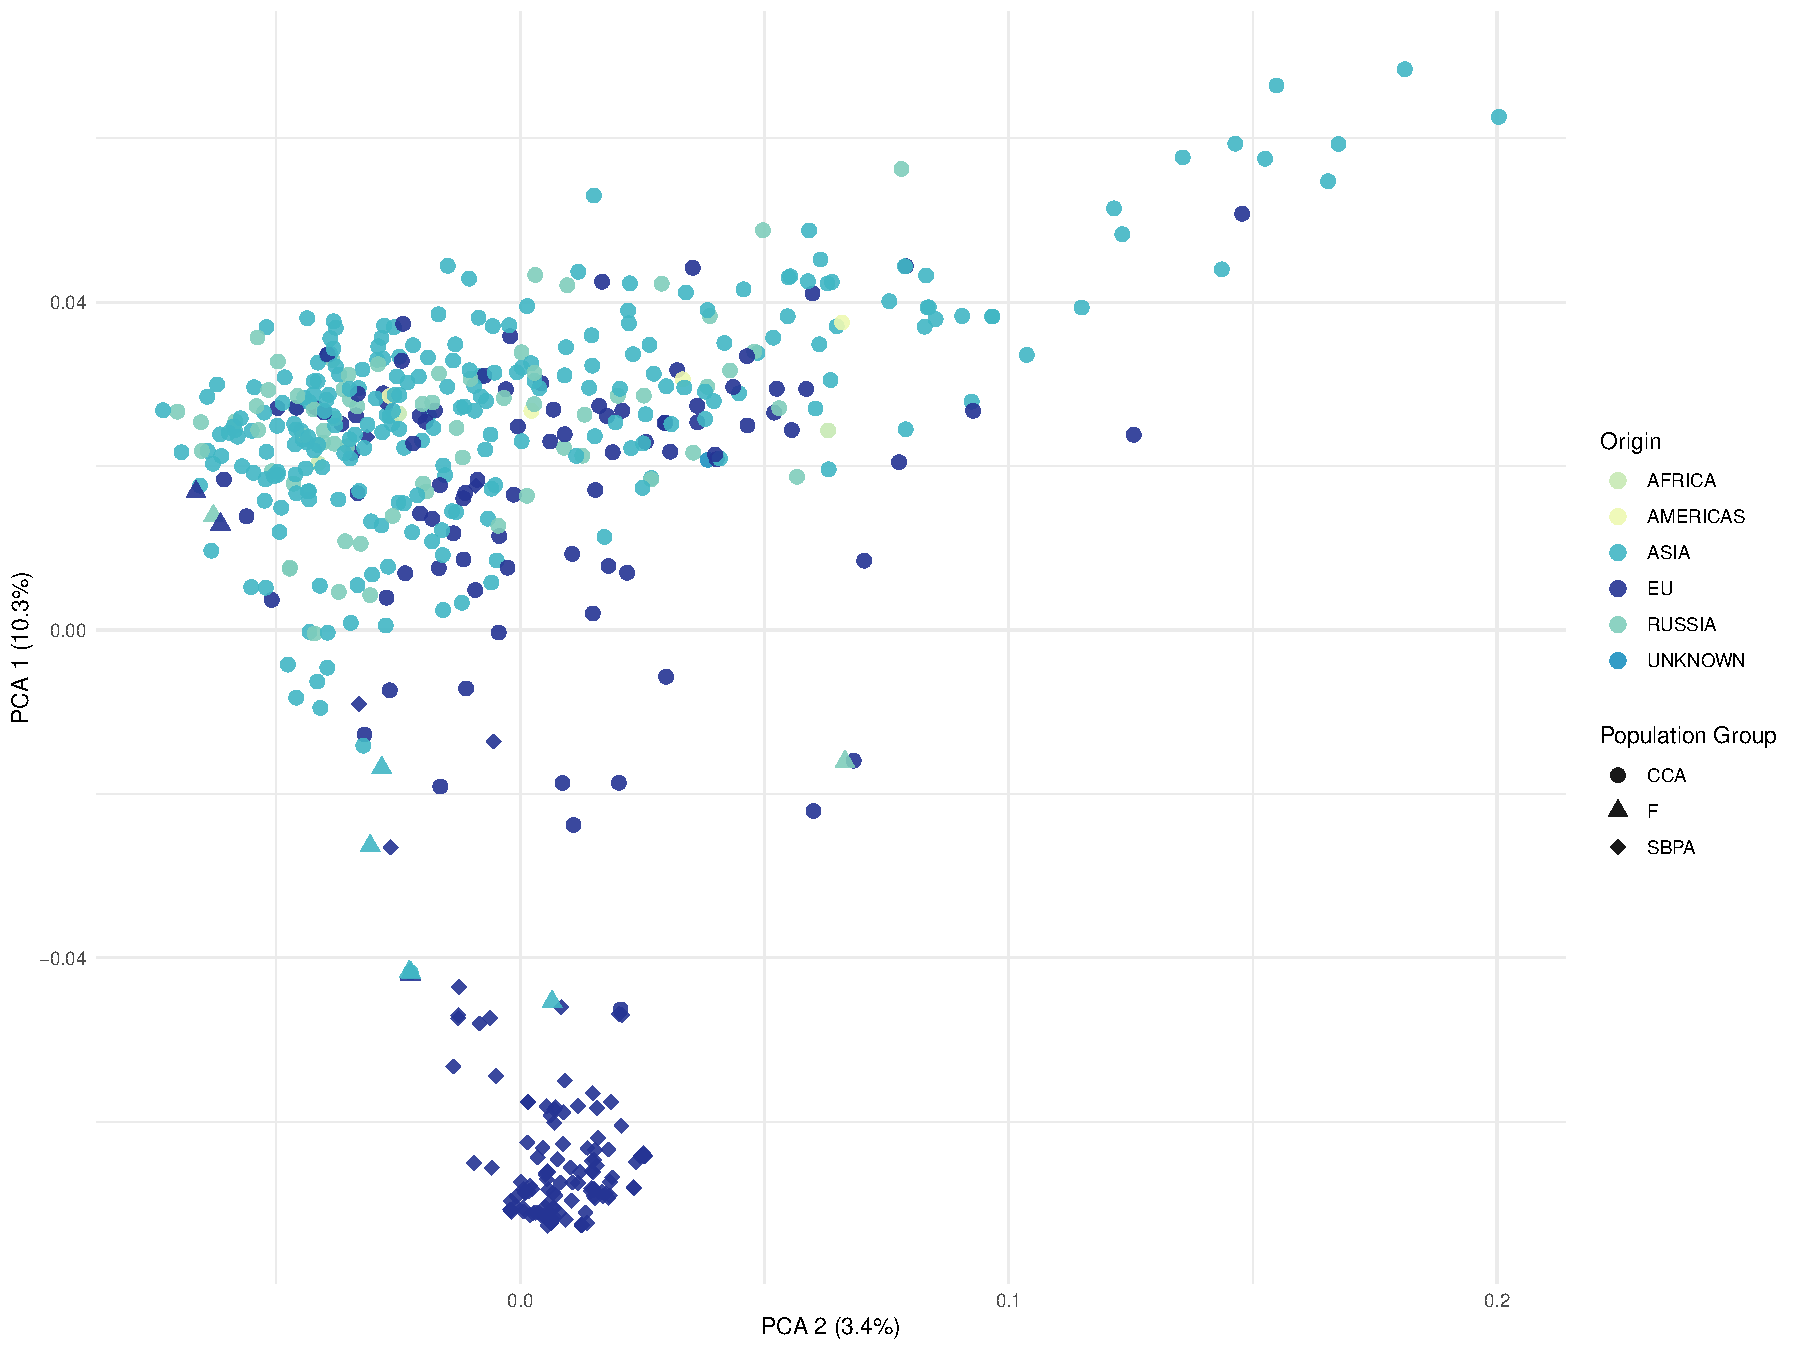
\includegraphics[width=\linewidth]{PCA1.pdf}
\caption{Biplot of the principal component analysis of soybean genotypes. The colours represent the defined origin groups, and the shapes indicate whether the accessions are from the Core Collection Accessions (CCA), the Swedish Breeding Program Accessions (SBPA) or the Founders of the breeding program (F).}
\label{fig:pca}
\end{figure}


\begin{figure}[p]
\centering
\includegraphics[width=\linewidth]{heat1.pdf}
\caption{This heatmap is a visual representation of the IBS values of the SBPA and CCA accessions. IBS values that are from 0 to 1 where 1 is identical by state. In the upper left corner are the SBPA accessions collected by the IBS matrix and hierarchical clustering-based analysis. The SBPA IBS values range from 0.73 to 0.97 for the SBPA and 0.56 to 0.98 for the CCA. The dataset as a whole, therefore ranges from 0.56 to 0.98.  }
\label{fig:heatall}
\end{figure}
\begin{figure}[p]
\centering
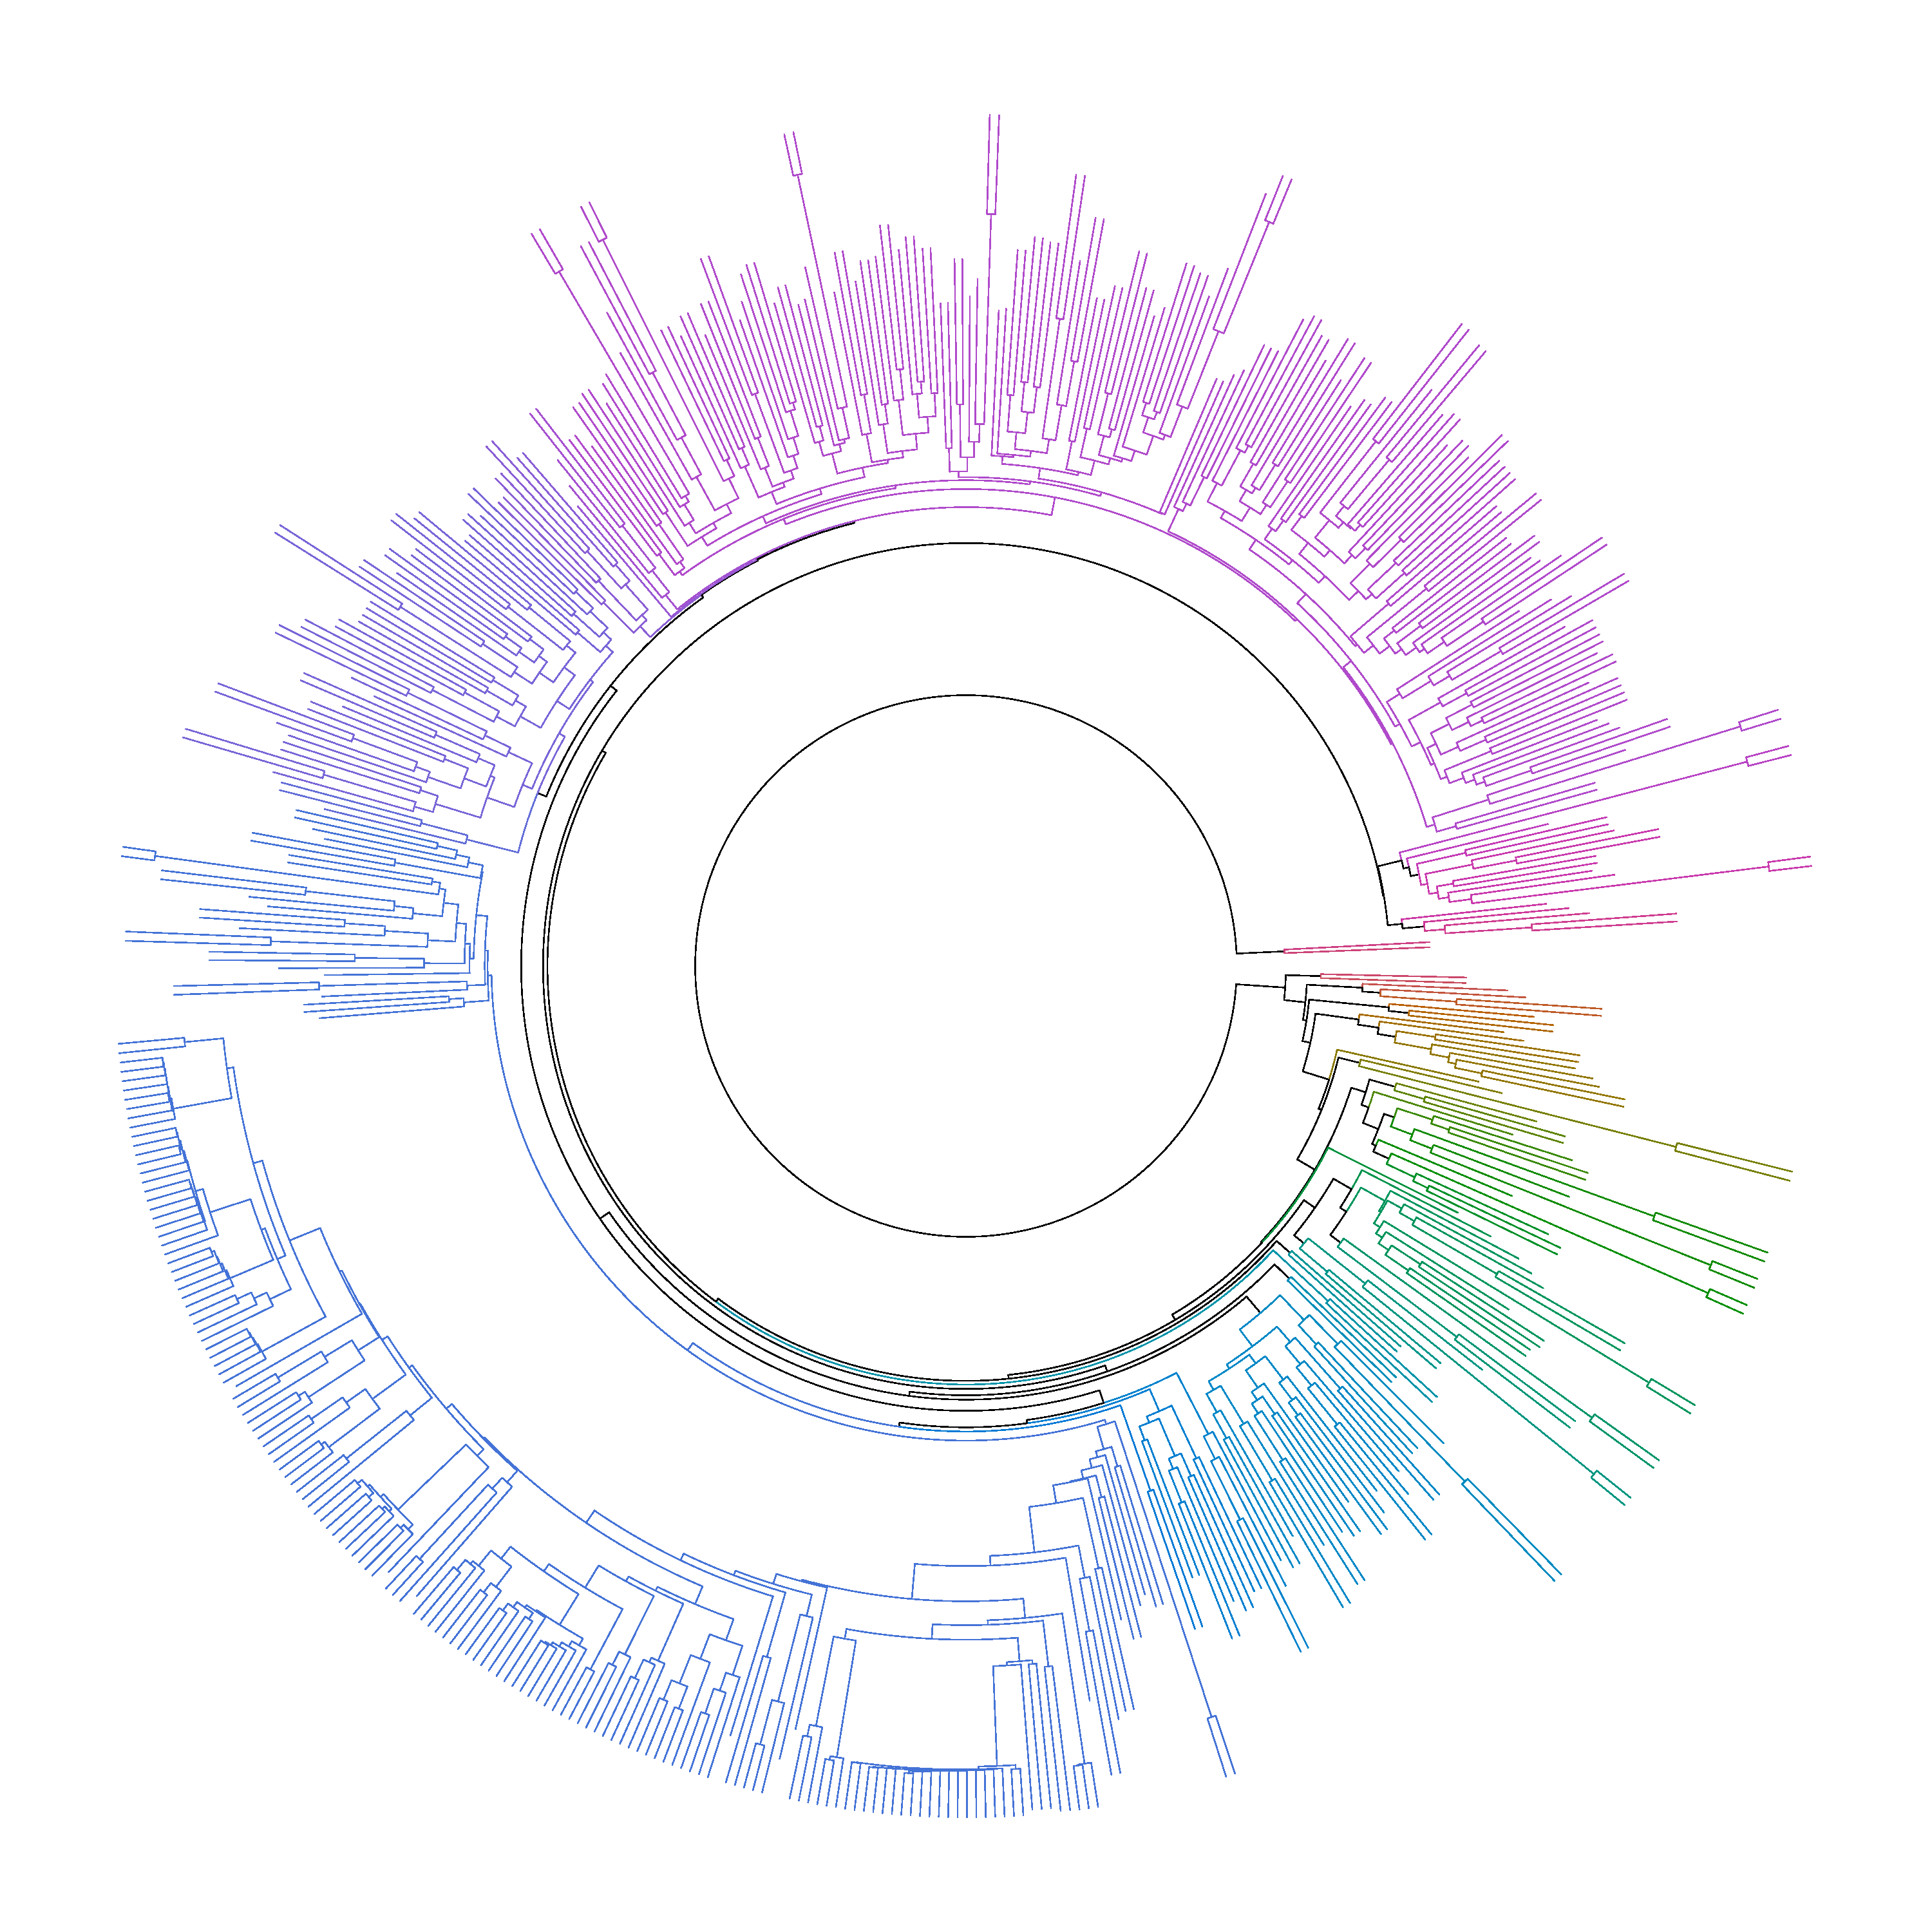
\includegraphics[width=\linewidth]{rainbow.pdf}

\caption{Hierarchical cluster dendrogram based on pairwise identity-by-state (IBS) values from the 50K SNP data for all samples. Including the suspected Founders. The dark blue accessions grouped together are a genetically cohesive group. Based on An IBS analysis is seen that the SBPA are genetically distinct from the other accessions, clustering together. Several Founders are seen clustering hierarchically outside the SBPA. The Swedish accessions Altonagård and Ugra Soja cluster outside }%
\label{fig:dendo}
\end{figure}


\begin{wraptable}{r}{0.5\textwidth}
\begin{table}[p]
\centering 
\caption{$F_{\text{ST}}$ estimation on genotypes. Measuring the population differentiation of  the 155 Accessions of the Nordgen genebank (Do again with only the 153 that were part of the breeding program)(SBPA) to the Core Collection of 409 accessions (CCA).}

\begin{tableminipage}{\textwidth}
\begin{tabular}{|l|l|l|l|l|l|l|}
\hline

Samples:                        &564        &          &          &          &          &          \\ \hline
SNPs:                           & 8,533,444 &          &          &          &          &          \\ \hline
Method: Weir \& Cockerham, 1984 &           &          &          &          &          &          \\ \hline
Populations:                  & CCA       & 409      & SBPA     & 155      &          &          \\ \hline
Weighted Fst estimate:          &0.2231884  &          &          &          &          &          \\ \hline
Mean Fst:                       &0.1108533  &          &          &          &          &          \\ \hline
summary:                        & Min.      & 1st Qu   & Median   & Mean     & 3rd Qu.  & Max.     \\ \hline
                                & -0.002515 & 0.011669 & 0.041730 & 0.110853 & 0.145697 & 0.975485 \\ \hline
\end{tabular}
  \label{tab:fst}
\end{tableminipage}
\end{table}
\end{wraptable}
\begin{wraptable}{r}{0.5\textwidth}
\begin{table}
\centering 
\caption{$F_{\text{ST}}$ estimation on Maturity groups, measuring the population differentiation of  the 155 Accessions of the Nordgen genebank that were part of the breeding program)(SBPA) to the Core Collection of 409 accessions (CCA) groups by the corrosponding maturity groups.}

\begin{tableminipage}{\textwidth}
\begin{tabular}{|l|c|l|l|l|l|l|l|l|l}
\cline{1-9}
\multicolumn{1}{|c|}{\begin{tabular}[c]{@{}c@{}}Weir and Cockerham \\ mean Fst estimate\end{tabular}} &
   &
  Group 1 &
  Group 2 &
  Group 3 &
  Group 4 &
  Group 5 &
  Group 6 &
  Group 7 &
   \\ \cline{1-9}
 &
  Maturity group &
  \multicolumn{1}{c|}{SBPA} &
  \multicolumn{1}{c|}{0-0-0} &
  \multicolumn{1}{c|}{0-0} &
  \multicolumn{1}{c|}{0} &
  \multicolumn{1}{c|}{I} &
  \multicolumn{1}{c|}{II - IV} &
  \multicolumn{1}{c|}{V - X} &
   \\ \cline{1-9}
Group 2 &
  0-0-0 &
  \cellcolor[HTML]{93CC7E}0.2968376 &
  \cellcolor[HTML]{E7E6E6} &
  \cellcolor[HTML]{E7E6E6} &
  \cellcolor[HTML]{E7E6E6} &
  \cellcolor[HTML]{E7E6E6} &
  \cellcolor[HTML]{E7E6E6} &
  \cellcolor[HTML]{E7E6E6} &
   \\ \cline{1-9}
Group 3 &
  0-0 &
  \cellcolor[HTML]{9FD07F}0.2702235 &
  \cellcolor[HTML]{FBAB77}0.0306470 &
  \cellcolor[HTML]{E7E6E6} &
  \cellcolor[HTML]{E7E6E6} &
  \cellcolor[HTML]{E7E6E6} &
  \cellcolor[HTML]{E7E6E6} &
  \cellcolor[HTML]{E7E6E6} &
   \\ \cline{1-9}
Group 4 &
  0 &
  \cellcolor[HTML]{B5D680}0.2212166 &
  \cellcolor[HTML]{FDCD7E}0.0428267 &
  \cellcolor[HTML]{F98B71}0.0191540 &
  \cellcolor[HTML]{E7E6E6} &
  \cellcolor[HTML]{E7E6E6} &
  \cellcolor[HTML]{E7E6E6} &
  \cellcolor[HTML]{E7E6E6} &
   \\ \cline{1-9}
Group 5 &
  I &
  \cellcolor[HTML]{B8D780}0.2146631 &
  \cellcolor[HTML]{FEE983}0.0525354 &
  \cellcolor[HTML]{FA9D75}0.0255972 &
  \cellcolor[HTML]{F8696B}0.0068046 &
  \cellcolor[HTML]{E7E6E6} &
  \cellcolor[HTML]{E7E6E6} &
  \cellcolor[HTML]{E7E6E6} &
   \\ \cline{1-9}
Group 6 &
  II - IV &
  \cellcolor[HTML]{8FCB7E}0.3063683 &
  \cellcolor[HTML]{FFEB84}0.0532384 &
  \cellcolor[HTML]{FCC27C}0.0387984 &
  \cellcolor[HTML]{FBA576}0.0282634 &
  \cellcolor[HTML]{FA9172}0.0212429 &
  \cellcolor[HTML]{E7E6E6} &
  \cellcolor[HTML]{E7E6E6} &
   \\ \cline{1-9}
Group 7 &
  V - X &
  \cellcolor[HTML]{63BE7B}0.4046471 &
  \cellcolor[HTML]{F6E984}0.0745305 &
  \cellcolor[HTML]{F7E984}0.0728984 &
  \cellcolor[HTML]{FCEB84}0.0607337 &
  \cellcolor[HTML]{FFEB84}0.0548296 &
  \cellcolor[HTML]{FBAA77}0.0301916 &
  \cellcolor[HTML]{E7E6E6} &
   \\ \cline{1-9}
\end{tabular}
  \label{tab:fst2}
\end{tableminipage}
\end{table}
\end{wraptable}



\subsection{H2 Low Genetic diversity and high LD decay in the SBPA point to a bottleneck and low Ne} 
There is a reduction in effective population size detected in a high level of linkage of the SBPA and a lower nucleotide diversity ($\pi$ ) in comparison to the CCA. There is also an accumulation of rare alleles and fixed alleles in the SBPA population. These observations suggest a bottleneck making an impact on the genetic composition of the SBPA population ensued by the intensification of genetic drift. 

\subsubsection{The SBP caused a bottleneck as seen in a decrease in genetic diversity }
Earlier studies have shown a halving in nucleotide diversity when comparing wild soybean to their domesticated progenitors and a further halving in nucleotide diversity in breeding regimes in recent years comparing landraces to elite cultivars \cite{kim21}. The SBPA have a mean nucleotide diversity of ($\pi$ = 0.000999), or a difference of  9/10.000 bases between two sequences. Whereas the CCA has almost double the mean nucleotide diversity of  ($\pi$ = 0.001911) or 19/10.000 bases differing.  The CCA has two times higher nucleotide diversity than the SBPA. This fall in nucleotide diversity is consistent with a bottleneck during the selection of founders and subsequent selection by the SBP.  

\subsubsection{Allele Frequency shows a high level of drift}
A high number of alleles at high frequency shows that the SBPA have a higher number of monomorphic locus than the CCA. A high number of fixed alleles together with the low nucleotide diversity can arise through natural selection, genetic bottlenecks, or genetic isolation in the population. The SBPA also has a higher number of genetic variants at low frequencies than the CCA Figure AF. Rare alleles arise through mutation, genetic drift, or migration from other populations. A high number of allele frequencies in the extremities of the frequency spectrum is a pattern of increased allel frequencies leading to fixation due to drift. Increased low freq allels can also be a signal of negative directional selection or a selective sweep, and an increase in high-frequency variants can be a signal of positive directional selection \cite{?}. 

\subsubsection{LD}
Figure \ref{fig:LD} shows a difference in LD over distance of the combined chromosomes. The decay of LD as measured by $r^2$ in the SBPA population and the CCA population. 







The presence of numerous rare alleles, seen in combination with the low pi and high decay, shows the genetic drift in the population. 
or

In conjuncture, the high number of rare alleles and high number of fixed alleles together reveal the bottleneck as also seen in the following LD decay analysis. 

We can deduce this since we know we are not looking at a diverse genetic pool, which could otherwise be a signal of a recent population expansion or balancing selection. Since we conclude that the accumulation of rare alleles is due to drift, we can assume that there is an accumulation of deleterious alleles in a population: The deleterious alleles can arise through spontaneous mutations and random fluctuations in allele frequencies, and the small size of the population leads to an increased frequency of harmful variants.

Although the findings above raise the possibility of potential selection processes occurring in the SBP, the high effect of genetic drift could mask any such signatures of selection making them indistinguishable because the drift enhances random fluctuations in  frequency making it difficult to detect or for the allele to reach fixation.



The next step is to predict if there are areas of the genome where the nucleotide diversity is lower than expected. 


The nonrandom association of alleles at different sites due to recombination (LD) in soybean shows like in the CCA
In this comparison of CCA and SBPA, we see a high LD at both low and high ranges of the SBPA. The LD slope of the SBPA shows a higher degree of decay over shorter physical distances, indicating in relation to the CCA, a contrasting population size. 

Longer range association estimates a small Ne, because of the bottleneck. 
The long-range LD will be due to a high level of fixation caused by drift.   

 

A difference in slope can also indicate different selective pressures or adaptive processes, such as the steep and higher slope of the SBPA may suggest positive selection or recent selective sweeps. 

AF 


\begin{figure}[p]
\centering
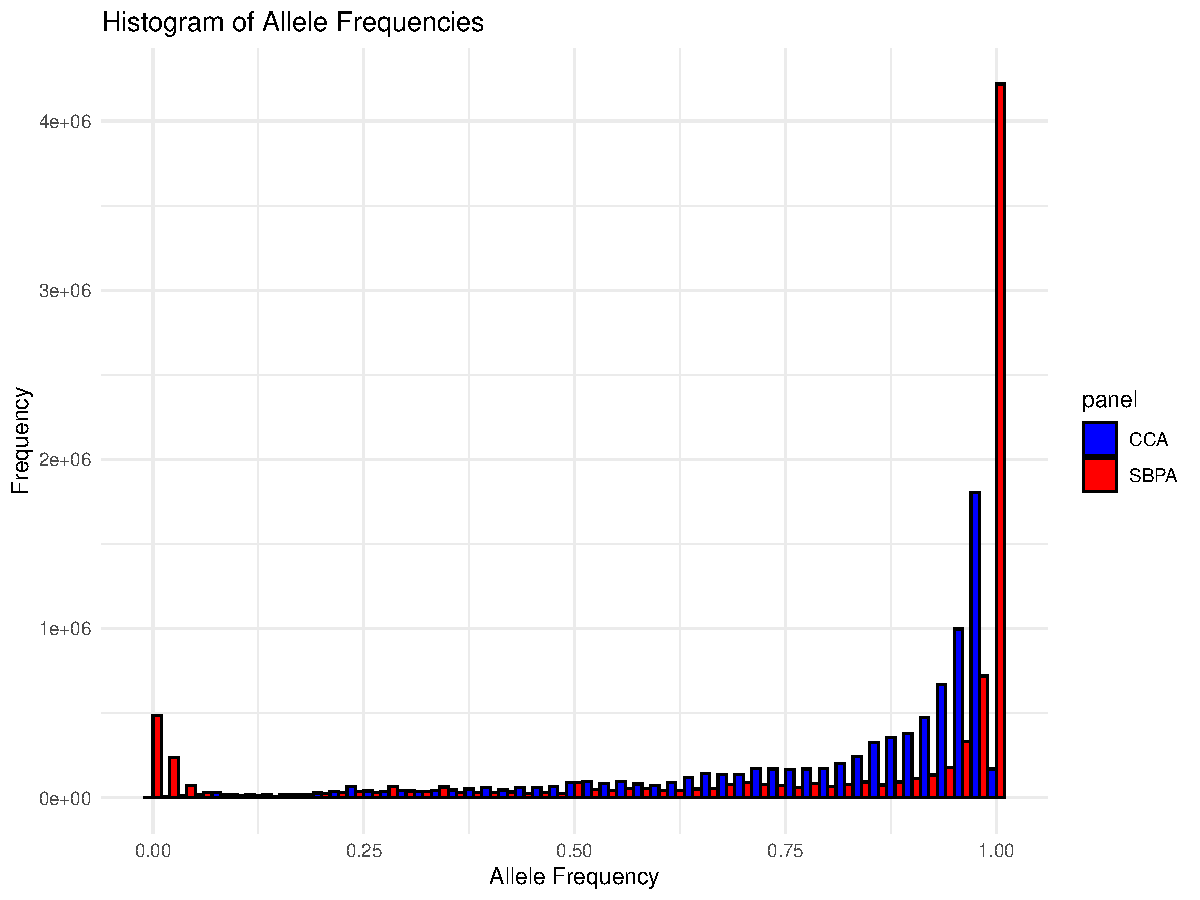
\includegraphics[width=\linewidth]{plot_AF.wgs.pdf}

\caption{Allele frequency distribition of the populations SBPA and CCA.  based on 8m snps with 1percent MAF filtered out. Comparing the two distrubutions }
\label{fig:AF}
\end{figure}
\begin{figure}[p]
\centering
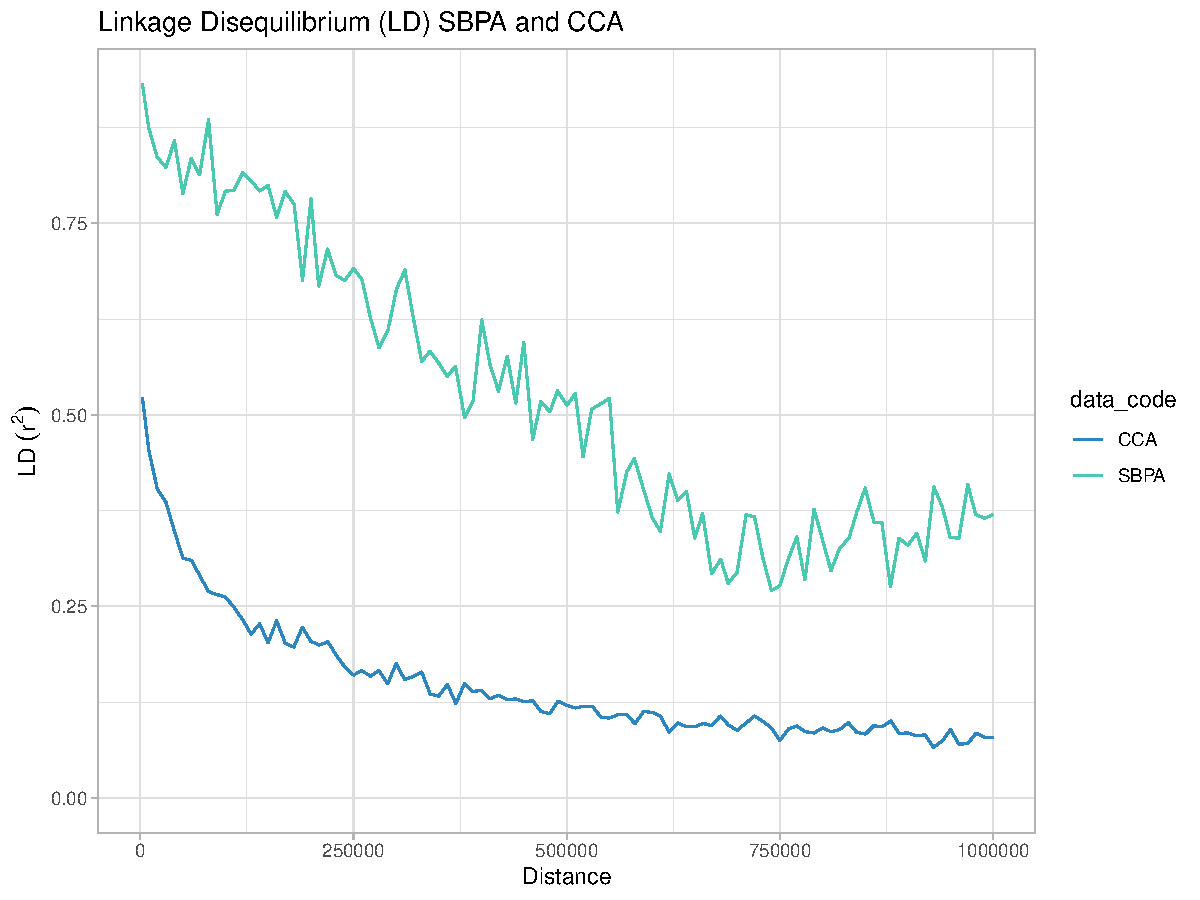
\includegraphics[width=\linewidth]{plot_LD_light.pdf}

\caption{LD decay ($r^2$) plotted against physical distance of the SNPs of the wgs data of aprox. 8 million SNPs. The mean value of $r^2$ was calculated in 10kb bins. The LD plot shows the relationship between genetic markers in the two populations at different sites due to recombination. The slope represents the rate at which LD decays with physical distance. The top cyan line is SBPA and the red line is the CCA. (If there is time i will include the slopes as vanlculated by the regression model)}

\label{fig:LD}
\end{figure}

\subsection{H3 Genome-wide selection signatures of vital pathways found to significant} 

Two methods of detecting selection in the genome was used. Tajimas D score was calculated on the SBPA population at 25kbp windows, detecting the non random values by  the measured and the expected values. Values under 0 are indicative of selection and this was the threshold used to test for a significant change in pathways for windows with genes where the amount was significanlty different from what was expected. using a fisheres exact test. Three pathways with a total of 443 genes in these pathways were shown to have been sigificant for degredated in the population; The Phospholipases pathway (lipasyn-pwy) and the Triacylglycerol Degradation pathway (lipasyn-pwy) are both involved in lipid metobilism.  Additionally the Aerobic Respiration I (Cytochrome C) (pwy-3781) which is an Mitocondria Energy pathway was significant. 

This is a signal that the degredation of these pathways has bean selected for. The Fst analysis showed no significants at these pathways but the odds ratio was towards degredation for the Triacylglycerol Degradation and Aerobic Respiration I (Cytochrome C) pathways. It is curious that pathways vital for respiration (such as Aerobic Respiration I involving Cytochrome C) and those involved in fatty acid and lipid biosynthesis and degradation (involving Phospholipases and Triacylglycerol Degradation) appear to have been selected against.
 
Fst scores calculated by a pairwise basepair comparison of the SBPA to the CCA was used with a threshold chosen at the topå 5\%. What we have discovered are colocalizations of regions exhibiting elevated Fst. Within these regions, we have conducted tests to provide evidence of recent sweeps. There are 34 pathways with a total of  where there is clear signal of gene enrichment. Interestingly these are essential plant metabolic pathways including primary metabolism where the differences are detected. See table Selection for the pathways and supplementary material for the genes in these pathways. For this analysis, all 34 pathways indicated enrichment. 
These pathways include; Amino Acid Metabolism; Carbohydrate Metabolism; Lipid Metabolism; Metabolism and Energy Production; Nucleotide Metabolism; Secondary Metabolism and Defense; And Vitamin and Cofactor Metabolism. see supplemetery matheral for the full overview of pathways and genes involved. 


\section{Discussion}

By combining population genetic and genomic methods the characterisation of the SBPA has shown that the selective breeding effort including founder selection has caused changes in the SBPA population. These changes are seen in light of the bottleneck effectuated on the population through the breeding program. We can infer that this bottleneck caused a decline in Ne and that drift acted strongly on the population, causing allele fixation. The selective breeding effort caused signatures of selection detected in this analysis, and its impact was observed primarily in key genetic pathways.

\textbf{Conclusion and Discussion H1} 
The evidence indicates a population stratification for the SBPA as a subpopulation and it is clear that the SBPA are a cohesive group in agreement with the IBS analysis clustering. The Fst analysis provides clarity on population stratification, revealing the SBPA as a distinct and identifiable subpopulation due to the high value of the fst. The PCA shows the SBPA grouped together due to their similarity.  The IBS calculation show the SBPA to be similar to each other and distinct from the CCA as a whole. 

It is expected that the SBPA would be seen as a subpopulation within the overall population using the CCA as a proxy of this. Comparing these results to previous work. Generally, a breeding program begins with a limited number of founders; these founders may have their own unique genetic backgrounds, and their genes will become prominent in the population over time. Crossing in the generations of the breeding program will function as inbreeding and diversity in the subpopulation will decrease over time. This has been seen in papers investigating both domestication and more recent breeding trajectories.  
What have others seen?
problems or shortcomings?
It was important for the further analyses of this research so as to avoid a confirmation bias loop that the SBPA was designated as a distinct subpopulation. This substantiated claim would then need to be supported by the PCA, IBS and Fst analysis to avoid circular reasoning in the next analyses.   
 
\textbf{H2 genetic diversity decline}

There is lower  genetic difference within the population of the 160 SBPA, as seen by the measure of nucleotide diversity. Essentially, this result indicates a high amount of genetic redundancy within the individuals of the population. This result is expected and follows the consequences of a breeding program where few founders are used, and the same founders (or offspring of crosses between these same founders) are continually recrossed into the breeding lines, effectuating inbreeding. This high similarity within the population was observed in the PCA and IBS analysis, the pi calculation confirms this and quantifies it. The explanation for the low nucleotide diversity is due to the initial diversity in the founders, the random drift caused by the small population size, and the common soybean breeding practices. Which are hybridisation to create variability for the breeder's selection followed by backcrossing and single seed decent. The practice of selfing the plants for several generations ensures homozygousity needed for seed suitable for cultivar distribution but further diminishes any diversity that was heterozygous \cite{acquaah12}. The assertion regarding the utilization of these breeding practices gains additional support from the pedigrees and historical documents detailing the breeding program and its outcomes, as presented in supplementary material S3 and referenced in  \cite{holmberg1973}.   

comparing these results to previous work, 
The CCA and them In relation to the GrinGlobal. USDA 

Discuss any problems or shortcomings encountered during the course of the work.
If i were to repeat this analysis i would have seen if there were any outgroups to comapre with. An  intersect was conducted of the 50K snp data and the wgs data to include founders for the PCA analysis , I could have included some glycine Sawyer and other glycine Max accessions, so as to have a better picture of the change in nucleotide diversity within the SBPA. It is also later come to light through investigation of historical documents and Gene Banks that there is a greater number of founders in the USD a 50 K snip datafuture analysis could include this larger number of founders so as to see the change from soybean diversity as a whole to the end nucleotide diversity change in the founders to the nucleotide genetic diversity change in the SBPE population. We are here by comparing the CCA to the SBPA debottleneck, affect or founder effect of the founders is in the data.  

\textbf{discussions \& conclusion H2 Bottleneck and Ne}
summarizing the results
High number of fixed and alleles in the SBPA population is s due to initial nucleotide diversity level and drift. 


analysis are well-supported and indicate certain characteristics of the SBPA population substantiated in the population assessment as a whole, this comprehensive examination of various aspects related to the SBPA as a population shown from several facets (name them) a population that has indeed gone through a bottleneck effectuating a small population size causing strong drift effects. 

LD
Linkage Disequalibrium is higher in the SBP a population than the CCA. The CCA linkage pattern is as in other soy diversity panels \cite{liu16}. The rate of decay or the slope of linkage seen can be directly compared can be a direct indication of effective population size is. It is therefore clear in figure \ref{fig:LD} that the SBPA population has a smaller effective population size than the CCA.
Genetic linkage is seen to increase the amount of genetic drift near any given locus thus reducing the effective population size. It is expected that a breeding screen would have the effect on a population such as the SBPA of higher correlation of alleles  at different loci than the CCA. Due to the limited number of recombination since the initial crosses of founders were created. Genetic drift will also create LD because of the random haplotypes drifting up in frequency.  
LD is related to effective population size by the fact that recombination rate and the value of the correlation coeeficient between allele counts $r^2$. The Linkage disequalibrium ($r^2$) that is calculated from the data and plotted can be fitted to a nonlinear regression model using least squares. 
$y_i=1/\alpha+\beta  c_i)  +e_i$
$slope = \alpha$

A method for inference of effective populationsize is:
$N_e = 1 / (2 * c * E(r^2) - 1)$
$c= recombination rate $
the LD can be replaced by the slope: 
$E(r^2) =\alpha$
$Ne = 1 / (2 * \alpha * c)$

These estimations are only valid under idealised conditions, but as the CCA and the SBPA both deviate from the conditions and one could speculate that they deviate in similar ways as they are of the same domesticated species undergoing similar human caused artificial selection. Therefor i conclude that slope and therefore the Ne of the two populations can be compaired. We can therefore conclude that the Ne of the SBPA is smaller that the CCA.    



AF
Drift is strong in a population with small Ne because effective population size is a statistical measure of how meny copies of a locus are effectivly segregating in the population, so 

We know that 

\textbf{discussions \& conclusion H3 Selection}
summarizing the results
We detected 34 different pathways, varying in primary importance to plant function, with a significant number of genes involved in selective sweeps. Additionally, we identified significance indicating selection against three additional pathways.


was this the expected result? No, not really, once it was clear that the Ne of the SBPA was small and drift, having a strong influence on the population that there would not be much signal detected. 
But other studies combining the population genomics (they did the fst sweeps similar to me) did also find evedence of lokal adaptation in aribidopsis \cite{price18}in soybean \cite{FIND} 
Do we see evidence of selection? 
yes
Are we looking in the right places?
Should we expect directional changes for these traits? or are part of these traits complex  traits 

Discuss signal detection
Signal. Population
Ne
selection pressure 

Discuss the data
sample size
time of the breeding program?

Discuss the method and whether or not it is able to detect what we want to know. 
Analysis choice
Threshold arbitrary
caveats


Conclusion and Implications
this study reports the characteristics of the SBPA population  
ramifications and such



Figure \ref{fig:pca2} .

\begin{figure}[t]
\centering
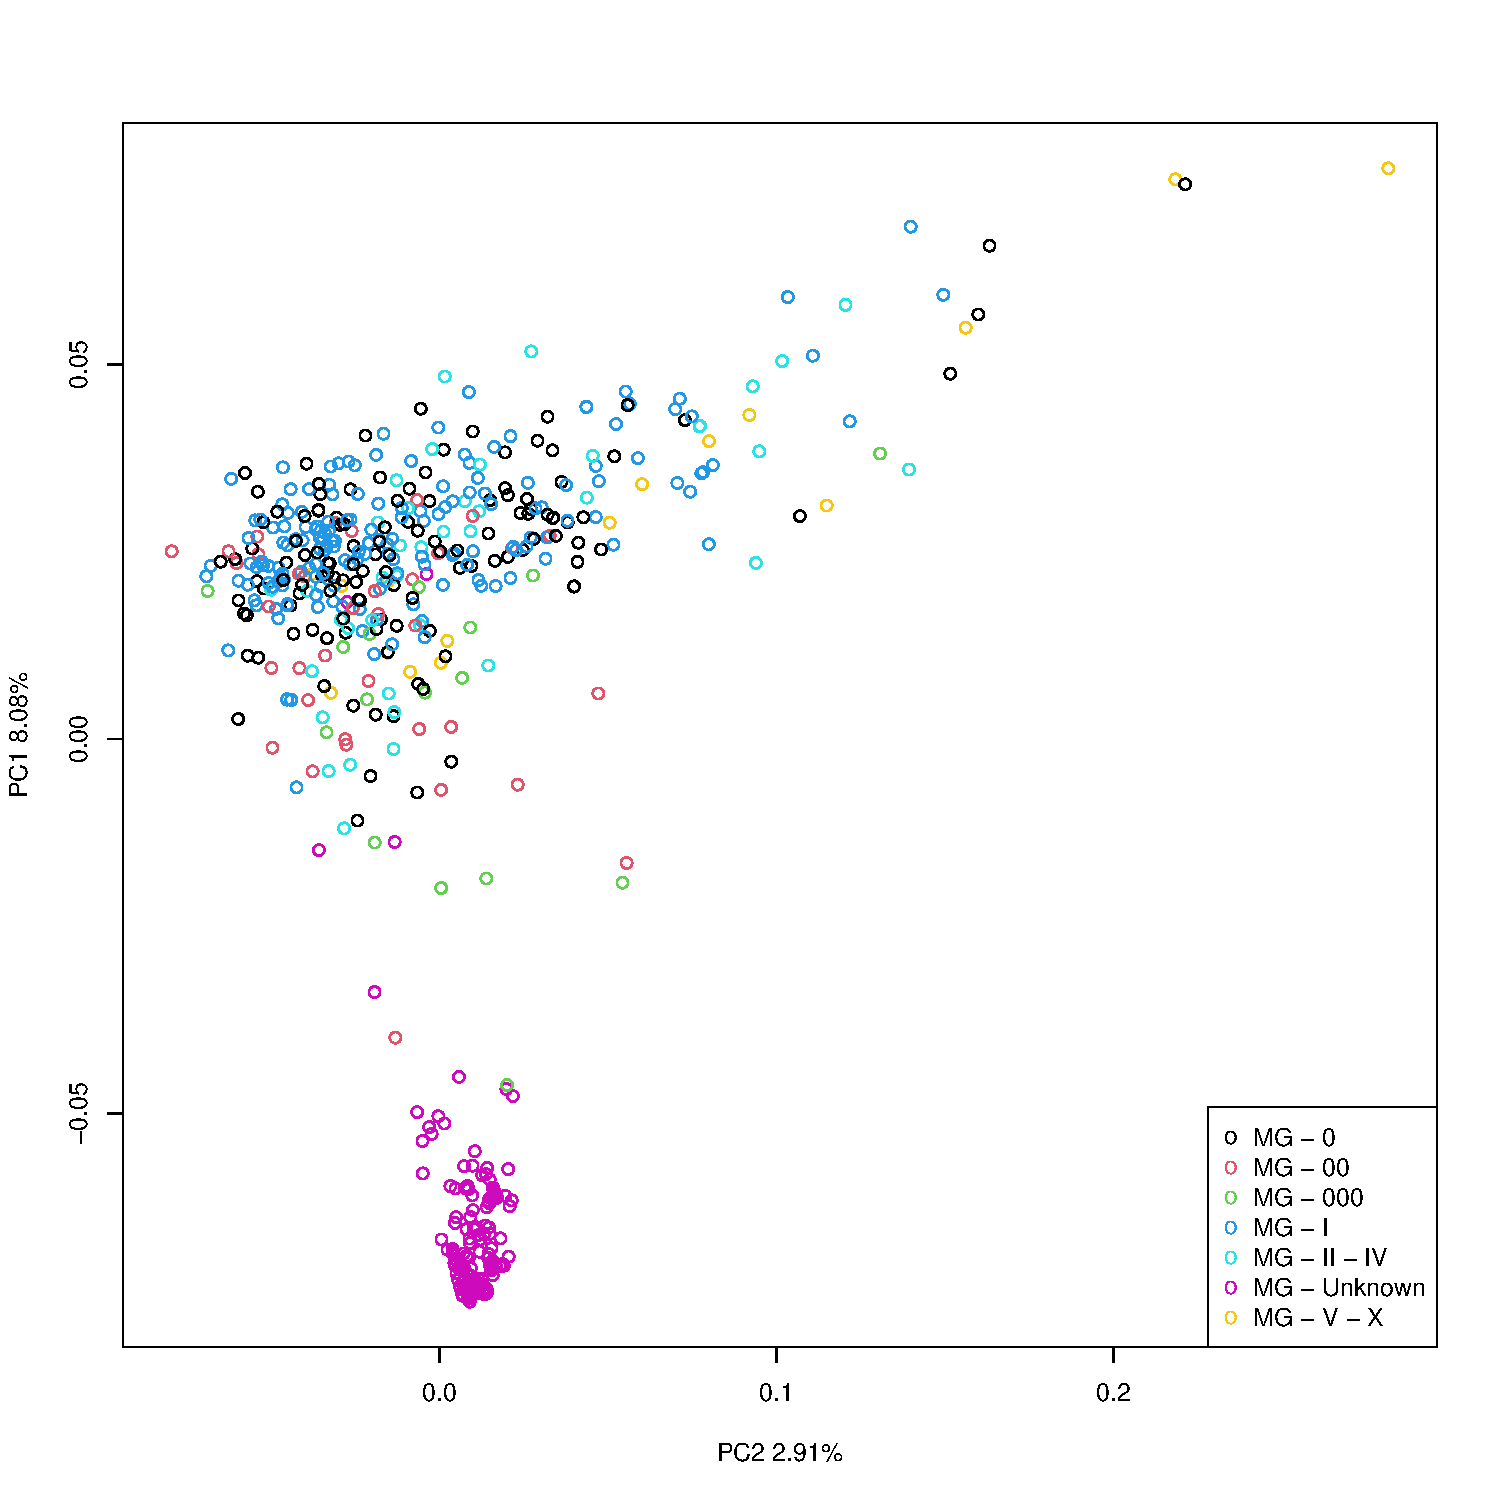
\includegraphics[width=\linewidth]{plot_PCA_mg1.pdf}
\caption{Principal component analysis for soybean samples from the whole genome sequence data, including the 155 Nordgen accessions and the 409 Core collection accessions. Indicated are the Maturity groups assigned to the accessions.}
\label{fig:pca2}
\end{figure}


\subsection{PCA3 figure}


Figure \ref{fig:pca3} .

\begin{figure}[t]
\centering
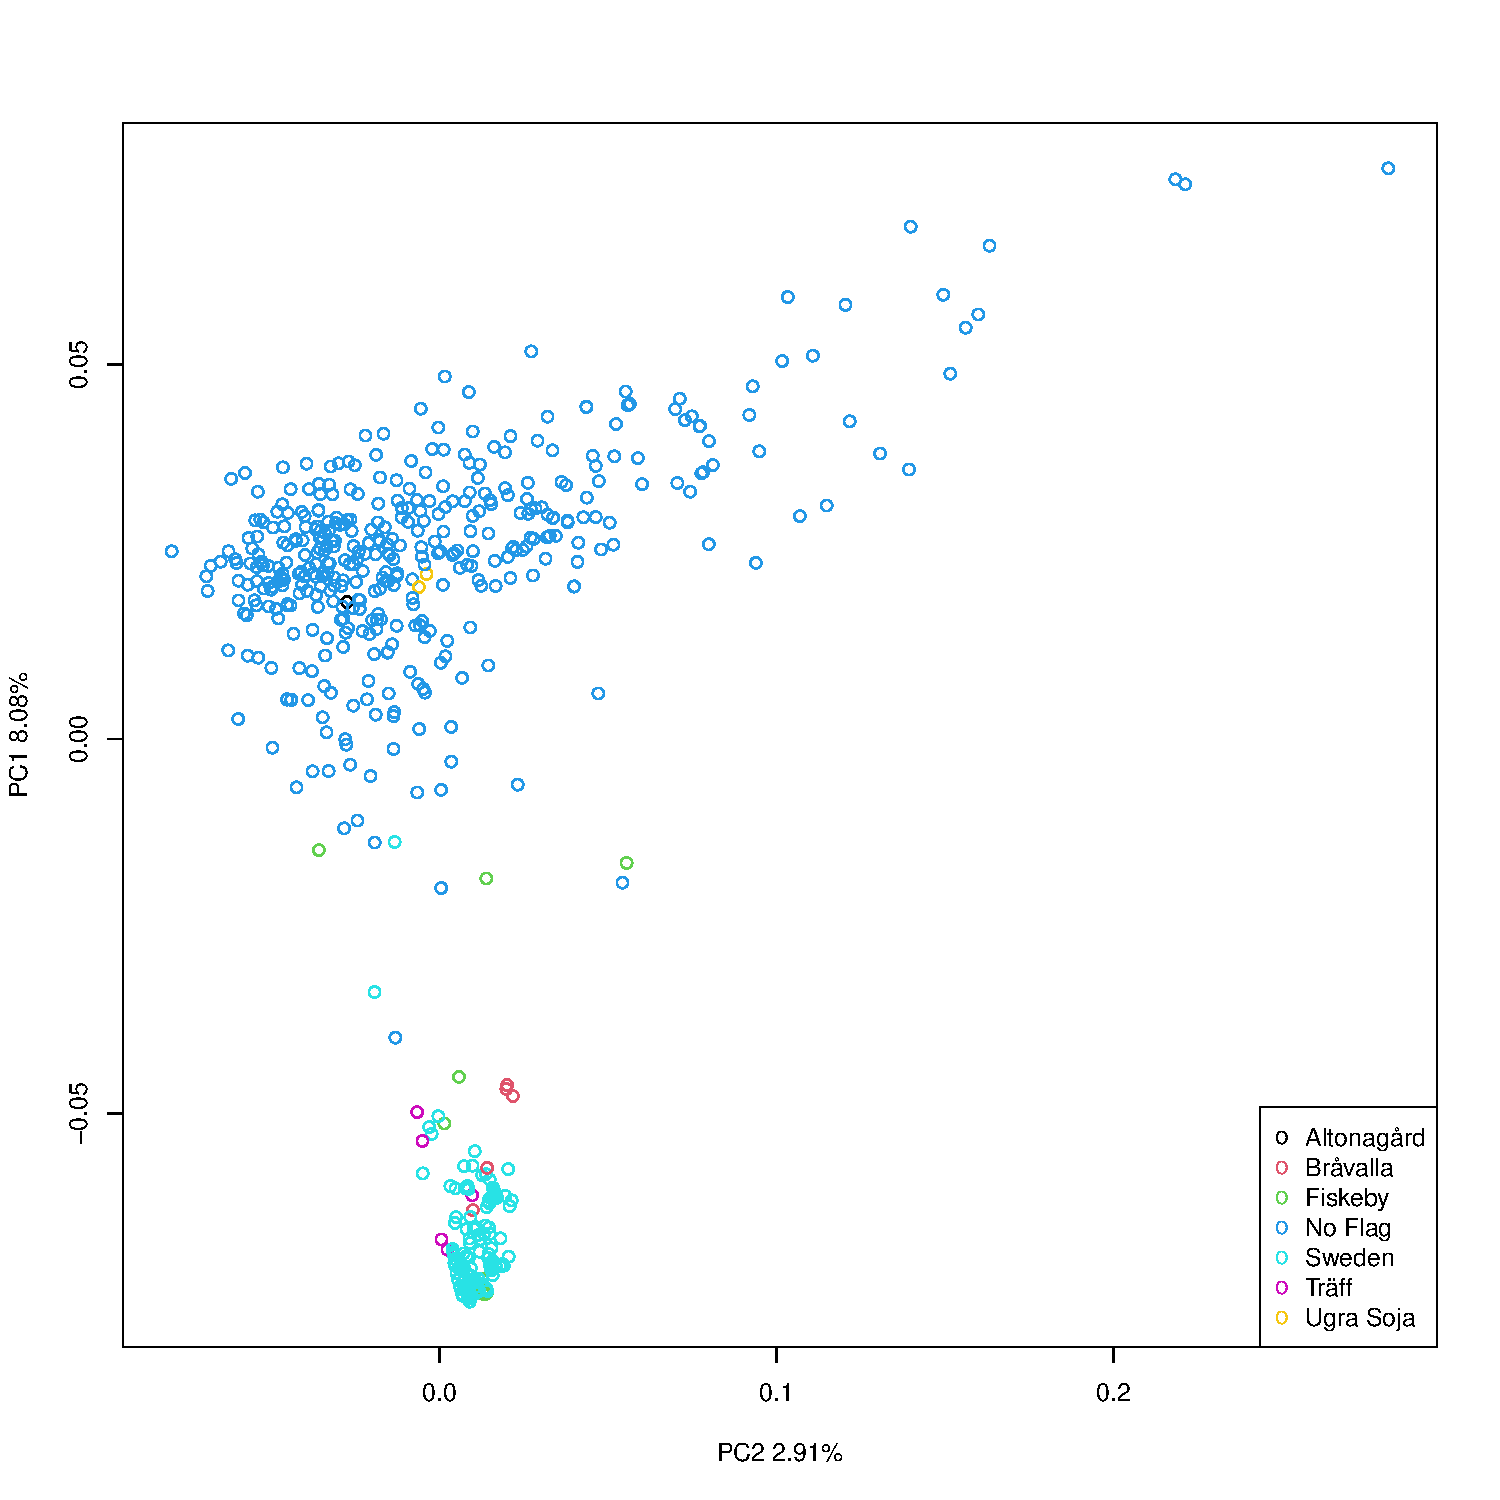
\includegraphics[width=\linewidth]{plot_PCA_flag.pdf}
\caption{PCA flag}
\label{fig:pca3}
\end{figure}



\subsection{PCA figure4}


Figure \ref{fig:pca4} .

\begin{figure}[t]
\centering
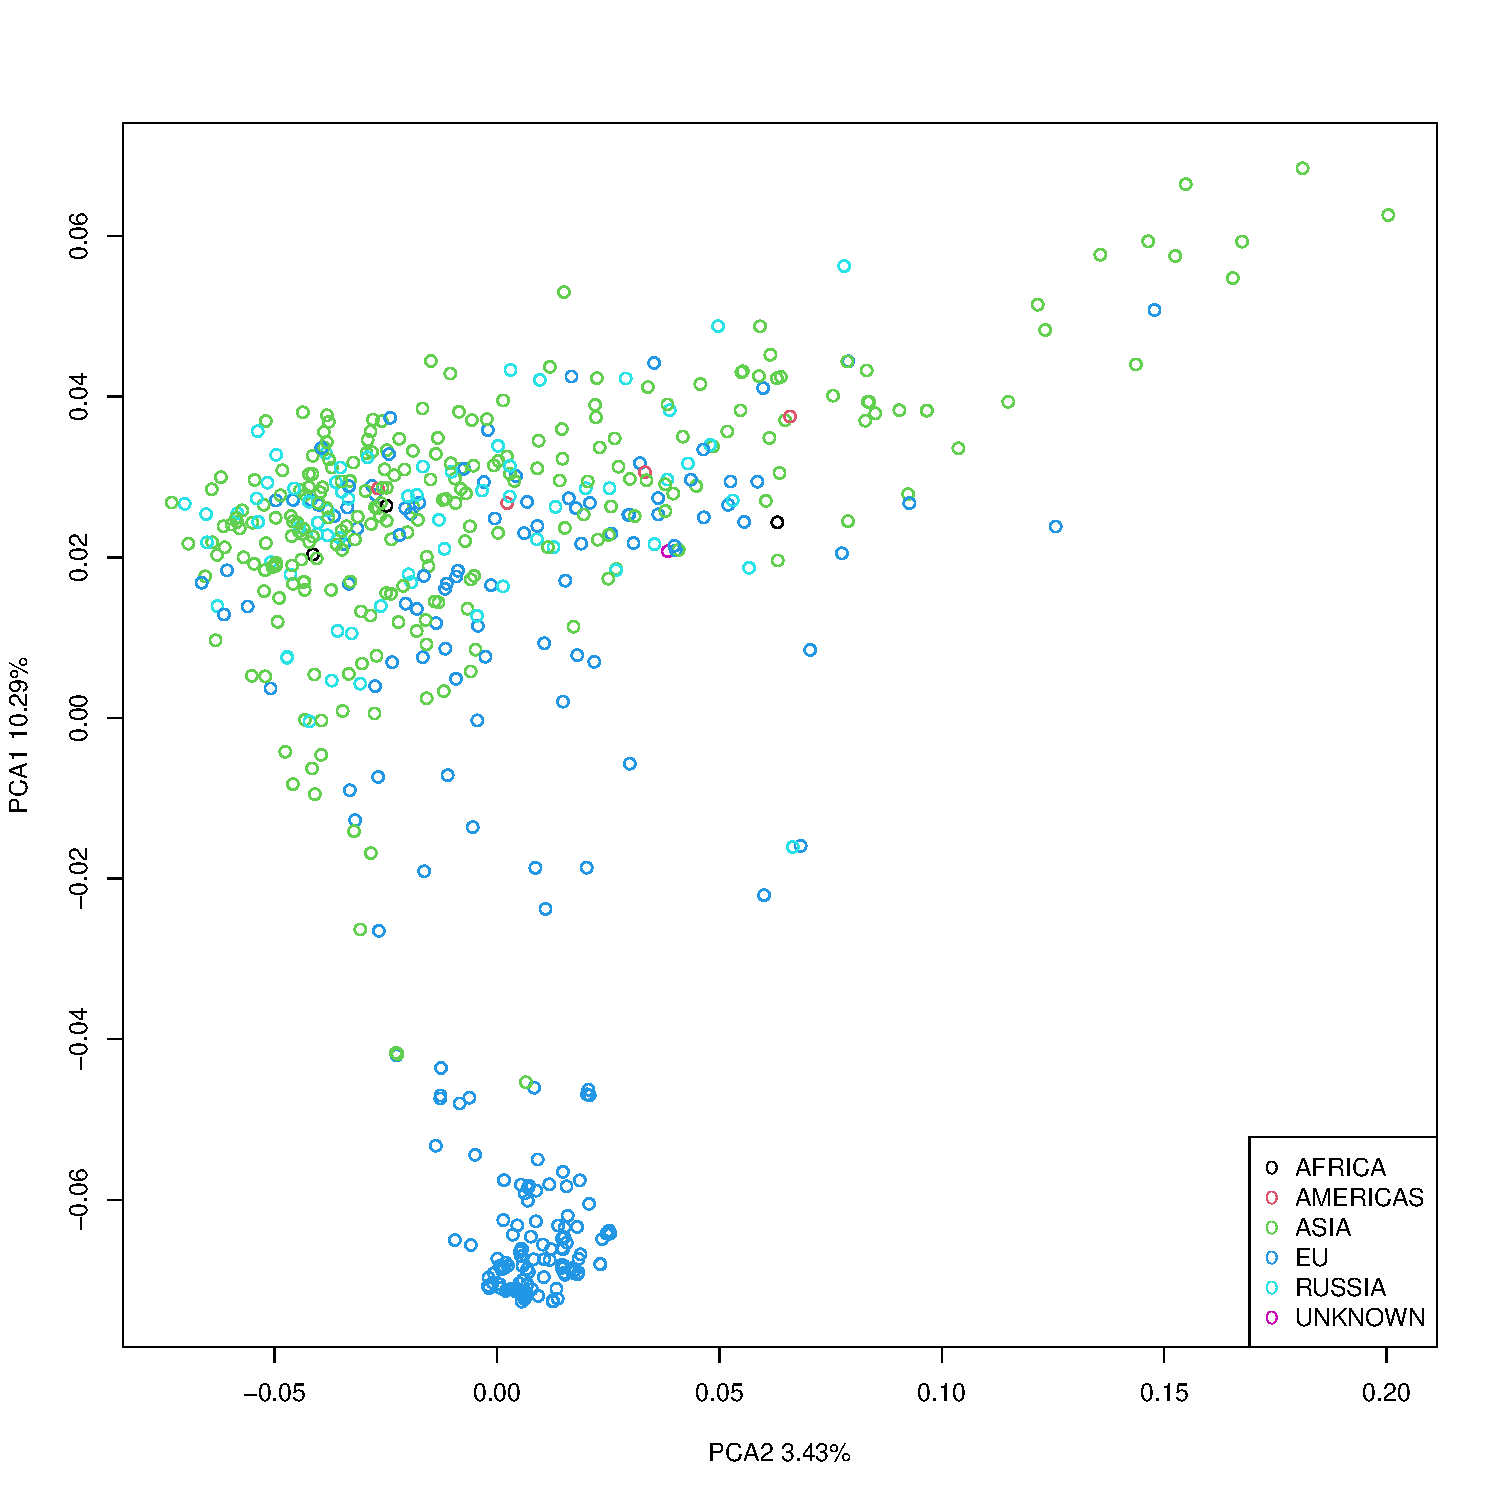
\includegraphics[width=\linewidth]{plot_PCA_region2.pdf}
\caption{PCA regions}
\label{fig:pca4}
\end{figure}


\begin{table}[p]
\centering 
\caption{$F_{\text{ST}}$ estimation on genotypes. Measuring the population differentiation of  the 155 Accessions of the Nordgen genebank (Do again with only the 153 that were part of the breeding program)(SBPA) to the Core Collection of 409 accessions (CCA).}

\begin{tableminipage}{\textwidth}
\begin{tabular}{|l|l|l|l|l|l|l|}
\hline

Samples:                        &564        &          &          &          &          &          \\ \hline
SNPs:                           & 8,533,444 &          &          &          &          &          \\ \hline
Method: Weir \& Cockerham, 1984 &           &          &          &          &          &          \\ \hline
Populations:                  & CCA       & 409      & SBPA     & 155      &          &          \\ \hline
Weighted Fst estimate:          &0.2231884  &          &          &          &          &          \\ \hline
Mean Fst:                       &0.1108533  &          &          &          &          &          \\ \hline
summary:                        & Min.      & 1st Qu   & Median   & Mean     & 3rd Qu.  & Max.     \\ \hline
                                & -0.002515 & 0.011669 & 0.041730 & 0.110853 & 0.145697 & 0.975485 \\ \hline
\end{tabular}
  \label{tab:fst}
\end{tableminipage}
\end{table}

\begin{table}[tb]
\centering 
\caption{$F_{\text{ST}}$ estimation on Maturity groups, measuring the population differentiation of  the 155 Accessions of the Nordgen genebank that were part of the breeding program)(SBPA) to the Core Collection of 409 accessions (CCA) groups by the corrosponding maturity groups.}

\begin{tableminipage}{\textwidth}
\begin{tabular}{|l|c|l|l|l|l|l|l|l|l}
\cline{1-9}
\multicolumn{1}{|c|}{\begin{tabular}[c]{@{}c@{}}Weir and Cockerham \\ mean Fst estimate\end{tabular}} &
   &
  Group 1 &
  Group 2 &
  Group 3 &
  Group 4 &
  Group 5 &
  Group 6 &
  Group 7 &
   \\ \cline{1-9}
 &
  Maturity group &
  \multicolumn{1}{c|}{SBPA} &
  \multicolumn{1}{c|}{0-0-0} &
  \multicolumn{1}{c|}{0-0} &
  \multicolumn{1}{c|}{0} &
  \multicolumn{1}{c|}{I} &
  \multicolumn{1}{c|}{II - IV} &
  \multicolumn{1}{c|}{V - X} &
   \\ \cline{1-9}
Group 2 &
  0-0-0 &
  \cellcolor[HTML]{93CC7E}0.2968376 &
  \cellcolor[HTML]{E7E6E6} &
  \cellcolor[HTML]{E7E6E6} &
  \cellcolor[HTML]{E7E6E6} &
  \cellcolor[HTML]{E7E6E6} &
  \cellcolor[HTML]{E7E6E6} &
  \cellcolor[HTML]{E7E6E6} &
   \\ \cline{1-9}
Group 3 &
  0-0 &
  \cellcolor[HTML]{9FD07F}0.2702235 &
  \cellcolor[HTML]{FBAB77}0.0306470 &
  \cellcolor[HTML]{E7E6E6} &
  \cellcolor[HTML]{E7E6E6} &
  \cellcolor[HTML]{E7E6E6} &
  \cellcolor[HTML]{E7E6E6} &
  \cellcolor[HTML]{E7E6E6} &
   \\ \cline{1-9}
Group 4 &
  0 &
  \cellcolor[HTML]{B5D680}0.2212166 &
  \cellcolor[HTML]{FDCD7E}0.0428267 &
  \cellcolor[HTML]{F98B71}0.0191540 &
  \cellcolor[HTML]{E7E6E6} &
  \cellcolor[HTML]{E7E6E6} &
  \cellcolor[HTML]{E7E6E6} &
  \cellcolor[HTML]{E7E6E6} &
   \\ \cline{1-9}
Group 5 &
  I &
  \cellcolor[HTML]{B8D780}0.2146631 &
  \cellcolor[HTML]{FEE983}0.0525354 &
  \cellcolor[HTML]{FA9D75}0.0255972 &
  \cellcolor[HTML]{F8696B}0.0068046 &
  \cellcolor[HTML]{E7E6E6} &
  \cellcolor[HTML]{E7E6E6} &
  \cellcolor[HTML]{E7E6E6} &
   \\ \cline{1-9}
Group 6 &
  II - IV &
  \cellcolor[HTML]{8FCB7E}0.3063683 &
  \cellcolor[HTML]{FFEB84}0.0532384 &
  \cellcolor[HTML]{FCC27C}0.0387984 &
  \cellcolor[HTML]{FBA576}0.0282634 &
  \cellcolor[HTML]{FA9172}0.0212429 &
  \cellcolor[HTML]{E7E6E6} &
  \cellcolor[HTML]{E7E6E6} &
   \\ \cline{1-9}
Group 7 &
  V - X &
  \cellcolor[HTML]{63BE7B}0.4046471 &
  \cellcolor[HTML]{F6E984}0.0745305 &
  \cellcolor[HTML]{F7E984}0.0728984 &
  \cellcolor[HTML]{FCEB84}0.0607337 &
  \cellcolor[HTML]{FFEB84}0.0548296 &
  \cellcolor[HTML]{FBAA77}0.0301916 &
  \cellcolor[HTML]{E7E6E6} &
   \\ \cline{1-9}
\end{tabular}
  \label{tab:fst2}
\end{tableminipage}
\end{table}


\section{Supplementary Material}
\label{sec:supplementary:material}

(S1: Overview) Detailed descriptions of all supplemental files. 
(S2: Accessions) Accession and pedigree data 
(S3: Methods 1) data preparation and filtering 
(S4: Methods 3) data analysis
(S5: Results)
(S6: Historical) Supplementary material historical information 

\subsection{Description of Supplementary Material}
File S1 contains detailed descriptions of all supplemental files. 
File S2 contains SNP ID numbers and locations. File S3 contains genotypes for each individual. Sequence data are available at GenBank and the accession numbers are listed in File S3. Gene expression data are available at GEO with the accession number: GDS1234. 

\section{Data availability}
\label{sec:data:availability}
For example: genotype data wgs are available upon request? 
File S1 contains detailed descriptions of all supplemental files. File S2 contains SNP ID numbers and locations. File S3 contains genotypes for each individual. Sequence data are available at GenBank and the accession numbers are listed in File S3. Gene expression data are available at GEO with the accession number: GDS1234. 
All code can be found at \url{https://github.com/JosephineConnelly/soyadapt_data_analysis}.

\section{Acknowledgments}
Acknowledgments should be included here.

\section{Funding}
Funding, including Funder Names and Grant numbers should be included here.

\section{Conflicts of interest}
There are  no known conflicts of interest.

add to file 
   @Manual{,
     title = {R: A Language and Environment for Statistical Computing},
     author = {{R Core Team}},
     organization = {R Foundation for Statistical Computing},
     address = {Vienna, Austria},
     year = {2021},
     url = {https://www.R-project.org/},
     }

\bibliography{bibliography}

    To insert a bibliography where bibfilename is the name of a .bib file.

\bibliographystyle{genetics}

        To choose a BibTeX bibliographic style file with the extension .bst.


\end{document} 